% ==================================================
% CHAPTER 6: The x-ray method
% ==================================================

\chapter{The x-ray method}
\label{chap:xray}

%TODO : consistently call the x-ray centroids the "x-ray beam profile centers"

Work on characterizing relative misalignments between quadruplet layers is ongoing~\cite{zhao_cosmic_2019}, \textcolor{red}{(Can I cite John's thesis-in-progress?)} but what is required are the absolute strip positions with respect to their nominal position in the ATLAS analysis coordinate system to be input into \package{Athena}~\cite{the_atlas_collaboration_athena}. Somehow, absolute misalignment parameters must be derived to create a model of absolute strip positions - which is not possible with the cosmics dataset. Absolute local offset measurements were done by the so-called x-ray method~\cite{lefebvre_precision_2020}. The x-ray tests were performed after the quadruplets arrived at CERN and were assembled into wedges. Essentially, an x-ray gun was attached to one of the source plates glued to the surface of the wedge (figure~\ref{fig:xray_setup}), and the beam profile recorded by the strips.

\begin{figure}
    \centering
    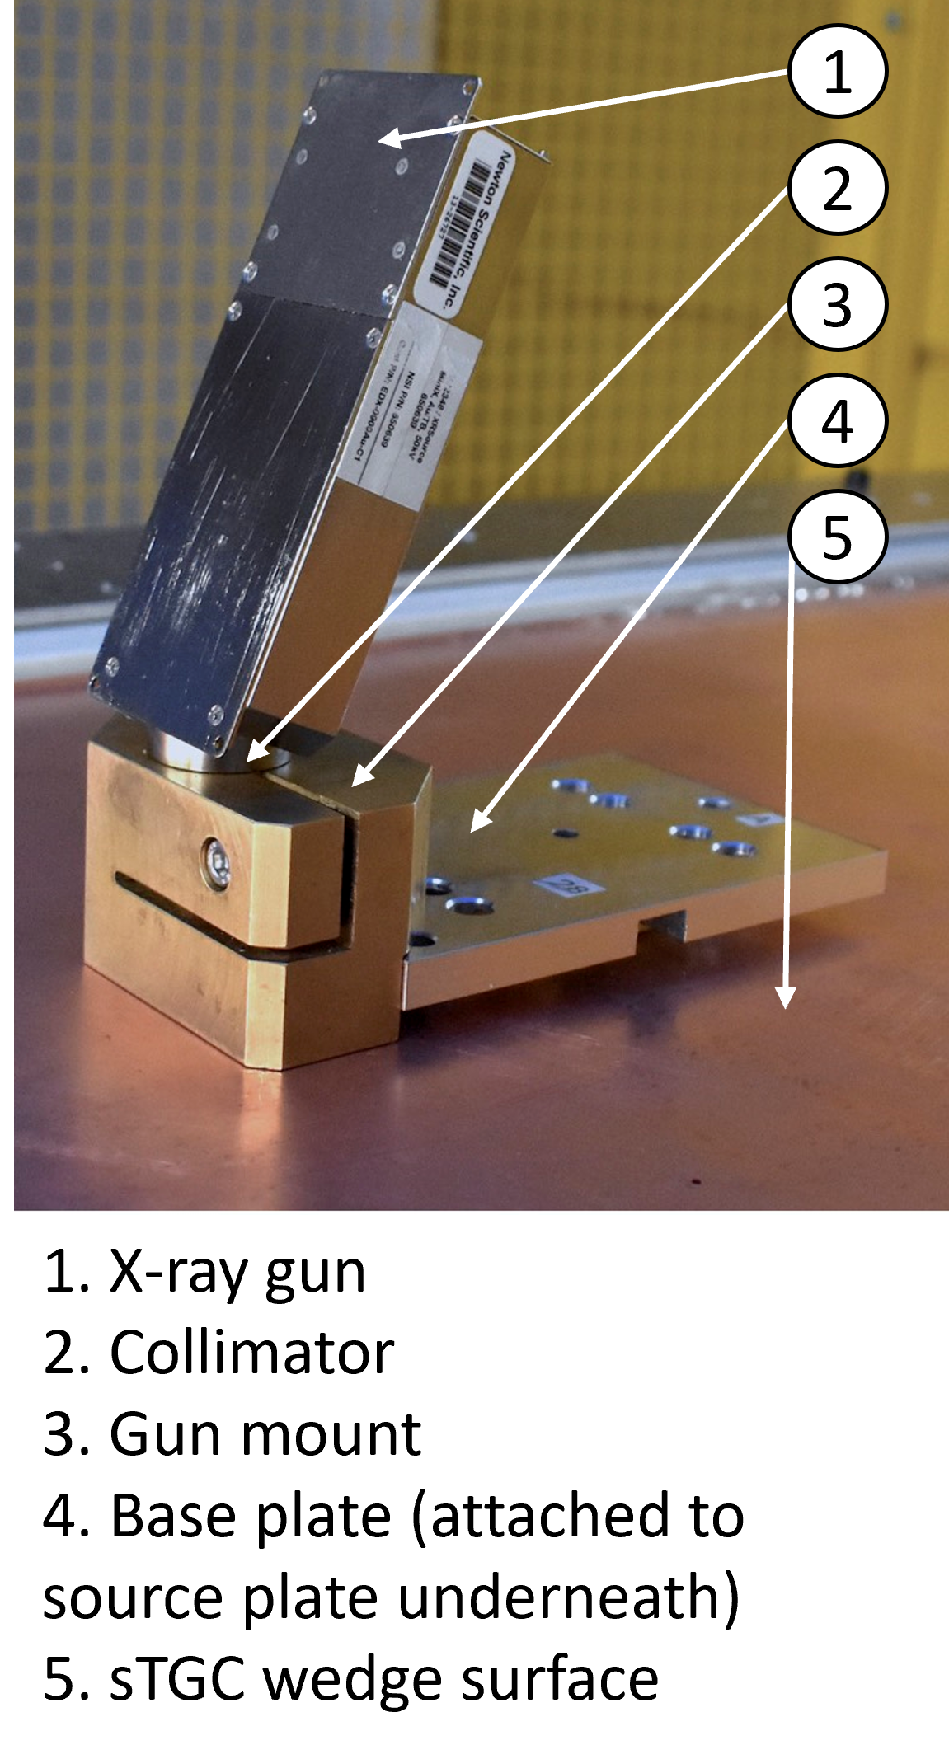
\includegraphics[width = 0.5\textwidth]{figures/figure_xray_setup.pdf}
    \caption{The x-ray gun mounted to the alignment platform on the surface of the wedge. Adapted from \copyright  CERN for the benefit of the ATLAS collaboration. CC-BY-4.0 license.}
    \label{fig:xray_setup}
\end{figure}

% During ATLAS operation, the position of the source plates will be monitored using the new alignment system~\cite{nsw_tdr}. Therefore, their position will be known in the absolute ATLAS coordinate system. 

The gun produced x-rays of 7 - \SI{15}{\kilo\electronvolt} that were collimated before reaching the surface of the wedge. The x-rays mostly interacted with the wedge's copper electrodes and gold-plated tungsten wires via the photo effect. The resulting photoelectrons caused ionization avalanches. The beam profile was captured by the distribution of cluster positions. A typical beam profile is shown in figure~\ref{fig:xray_beam_profile}.

\begin{figure}
    \centering
    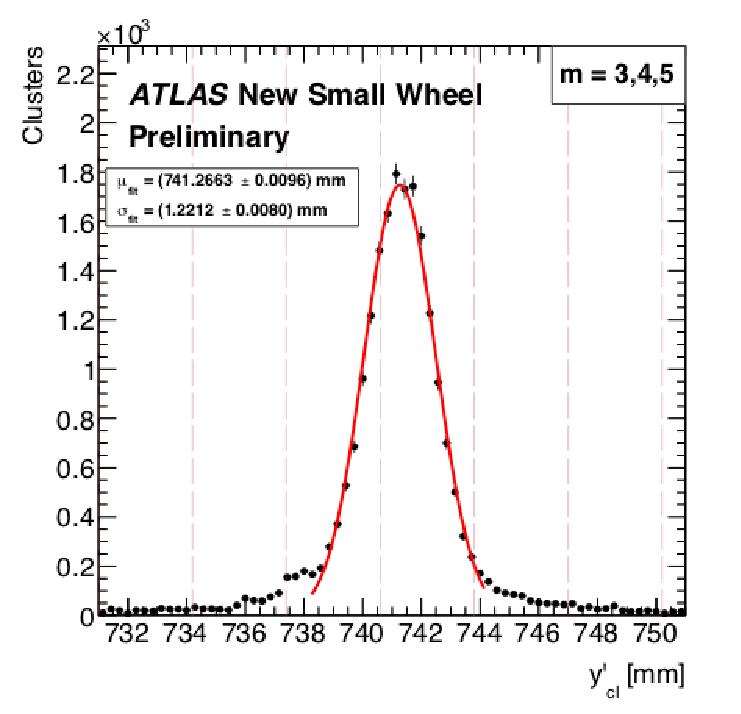
\includegraphics[width = 0.5\textwidth]{figures/figure_xray_beam_profile.pdf}
    \caption{Distribution of x-ray cluster mean positions after the analysis cuts and corrections. The strip cluster multiplicity, $m$, was limited to 3, 4 and 5. The red line is a Gaussian fit of the distribution and the pink lines denote the edges of the strips. Adapted from \copyright CERN for the benefit of the ATLAS collaboration. CC-BY-4.0 license.}
    \label{fig:xray_beam_profile}
\end{figure}

Clusters with signal on more than 5 strips were cut because they were most likely caused by photoelectrons ejected with enough energy to cause more primary ionization and subsequent avalanches ($\delta$-rays)~\cite{lefebvre_precision_2020}.

The mean of the cluster position distribution was taken as the x-ray beam profile center. The expected center was calculated assuming a wedge with nominal geometry given the gun position. The difference between the expected and reconstructed beam profile center is a measure of the local offset. Applying the logic of equation~\ref{eqn:local_translation} to the beam profile, the fitted mean acts as $y$, the expected center is $y_{nom}$ and the local offset is $d_{local}$ as before. The x-ray local offsets  give the absolute local position of the strip pattern with respect to the source plates. Since the position of the source plates will be monitored by the alignment system in ATLAS~\cite{nsw_tdr}, the local position of the strip pattern can be known in the ATLAS coordinate system for every position where x-ray data was taken.

%TODO : Maybe move this paragraph to start of comparison chapter
The main advantage of the x-ray dataset over the cosmics dataset is that absolute local offsets are measurable thanks to the reference frame provided by the source plates. However, the systematic uncertainty on the x-ray offsets is large: \SI{120}{\micro\meter} was accepted by the collaboration. The cuts and corrections applied to the x-ray data that motivate the uncertainty are detailed in Lefebvre, 2020~\cite{lefebvre_precision_2020}. In addition, local offset measurements were limited to the positions of the alignment platforms; only 10 - 20 positions were surveyed for each wedge. Therefore, validating the x-ray measurements and seeing how they can be improved is important because of the uncertainty in and incompleteness of the dataset. How the cosmics dataset was used for this purpose is discussed in chapter~\ref{chap:comparison}. 